% Options for packages loaded elsewhere
\PassOptionsToPackage{unicode}{hyperref}
\PassOptionsToPackage{hyphens}{url}
\PassOptionsToPackage{dvipsnames,svgnames,x11names}{xcolor}
%
\documentclass[
  11pt,
  a4paperpaper,
  onecolumn]{article}

\usepackage{amsmath,amssymb}
\usepackage{lmodern}
\usepackage{iftex}
\ifPDFTeX
  \usepackage[T1]{fontenc}
  \usepackage[utf8]{inputenc}
  \usepackage{textcomp} % provide euro and other symbols
\else % if luatex or xetex
  \usepackage{unicode-math}
  \defaultfontfeatures{Scale=MatchLowercase}
  \defaultfontfeatures[\rmfamily]{Ligatures=TeX,Scale=1}
\fi
% Use upquote if available, for straight quotes in verbatim environments
\IfFileExists{upquote.sty}{\usepackage{upquote}}{}
\IfFileExists{microtype.sty}{% use microtype if available
  \usepackage[]{microtype}
  \UseMicrotypeSet[protrusion]{basicmath} % disable protrusion for tt fonts
}{}
\makeatletter
\@ifundefined{KOMAClassName}{% if non-KOMA class
  \IfFileExists{parskip.sty}{%
    \usepackage{parskip}
  }{% else
    \setlength{\parindent}{0pt}
    \setlength{\parskip}{6pt plus 2pt minus 1pt}}
}{% if KOMA class
  \KOMAoptions{parskip=half}}
\makeatother
\usepackage{xcolor}
\usepackage[left=2cm,top=1.5cm,right=2cm,bottom=1.5cm]{geometry}
\setlength{\emergencystretch}{3em} % prevent overfull lines
\setcounter{secnumdepth}{-\maxdimen} % remove section numbering
% Make \paragraph and \subparagraph free-standing
\ifx\paragraph\undefined\else
  \let\oldparagraph\paragraph
  \renewcommand{\paragraph}[1]{\oldparagraph{#1}\mbox{}}
\fi
\ifx\subparagraph\undefined\else
  \let\oldsubparagraph\subparagraph
  \renewcommand{\subparagraph}[1]{\oldsubparagraph{#1}\mbox{}}
\fi


\providecommand{\tightlist}{%
  \setlength{\itemsep}{0pt}\setlength{\parskip}{0pt}}\usepackage{longtable,booktabs,array}
\usepackage{calc} % for calculating minipage widths
% Correct order of tables after \paragraph or \subparagraph
\usepackage{etoolbox}
\makeatletter
\patchcmd\longtable{\par}{\if@noskipsec\mbox{}\fi\par}{}{}
\makeatother
% Allow footnotes in longtable head/foot
\IfFileExists{footnotehyper.sty}{\usepackage{footnotehyper}}{\usepackage{footnote}}
\makesavenoteenv{longtable}
\usepackage{graphicx}
\makeatletter
\def\maxwidth{\ifdim\Gin@nat@width>\linewidth\linewidth\else\Gin@nat@width\fi}
\def\maxheight{\ifdim\Gin@nat@height>\textheight\textheight\else\Gin@nat@height\fi}
\makeatother
% Scale images if necessary, so that they will not overflow the page
% margins by default, and it is still possible to overwrite the defaults
% using explicit options in \includegraphics[width, height, ...]{}
\setkeys{Gin}{width=\maxwidth,height=\maxheight,keepaspectratio}
% Set default figure placement to htbp
\makeatletter
\def\fps@figure{htbp}
\makeatother
\newlength{\cslhangindent}
\setlength{\cslhangindent}{1.5em}
\newlength{\csllabelwidth}
\setlength{\csllabelwidth}{3em}
\newlength{\cslentryspacingunit} % times entry-spacing
\setlength{\cslentryspacingunit}{\parskip}
\newenvironment{CSLReferences}[2] % #1 hanging-ident, #2 entry spacing
 {% don't indent paragraphs
  \setlength{\parindent}{0pt}
  % turn on hanging indent if param 1 is 1
  \ifodd #1
  \let\oldpar\par
  \def\par{\hangindent=\cslhangindent\oldpar}
  \fi
  % set entry spacing
  \setlength{\parskip}{#2\cslentryspacingunit}
 }%
 {}
\usepackage{calc}
\newcommand{\CSLBlock}[1]{#1\hfill\break}
\newcommand{\CSLLeftMargin}[1]{\parbox[t]{\csllabelwidth}{#1}}
\newcommand{\CSLRightInline}[1]{\parbox[t]{\linewidth - \csllabelwidth}{#1}\break}
\newcommand{\CSLIndent}[1]{\hspace{\cslhangindent}#1}

%----------------------------------------------------
% 	CONFIGURATION OF PARAMETERS
%----------------------------------------------------
% ----------------
%  FONTS AND TYPESETTING SETTINGS
% -----------------
\usepackage[english]{babel}
%\usepackage[bitstream-charter]{mathdesign}
%use\usepackage{times}
\usepackage{fontawesome5}
\usepackage{academicons}
\usepackage[notransparent]{svg}
\usepackage{tabu}
%\usepackage{coloremoji}
%\usepackage{emoji}

\usepackage{longtable}

%\usepackage[tracking=smallcaps]{microtype}
%\usepackage[bitstream-charter]{mathdesign}

% ----------------
%  STYLES OF THE CHAPTER, SECTION
% -----------------
%Options: Sonny, Lenny, Glenn, Conny, Rejne, Bjarne, Bjornstrup
%\usepackage[Bjornstrup]{fncychap}
\usepackage{marginnote}
\renewcommand*{\marginfont}{\small\sffamily}
\usepackage{wrapfig}
\usepackage{floatflt}
  
%---------------------------------
% Modification du model de UL
%\graphicspath{{./Figures/}} % chemin des figures


% -----------------
%  DEFINITION OF THE COLORS
% -----------------
%\usepackage{color} % Color
%\usepackage[usenames,dvipsnames,table]{xcolor}
%\usepackage{colortbl}

% -----------------
% 	MATHEMATHICAL SYMBOLS
% -----------------
%\usepackage{amssymb} %% The amssymb package provides various useful mathematical symbols
%\usepackage{amsthm} %% The amsthm package provides extended theorem environments
%\usepackage{amsmath}  % Paqute de Matematicas
%----------------------------------------------------------------------------------------

% -----------------
%  BIBLIOGRAPHY
% -----------------
%\usepackage  {natbib}
\usepackage{csquotes} %a utiliser si biblatex est utilisé
%\usepackage[style=numeric-comp, doi=false, backend=bibtex, isbn=false, url=false, sorting=none, language=english ]{biblatex}
%\addbibresource{library.bib}

%\usepackage[toc,page]{appendix}
\usepackage{booktabs}
% -----------------
%  VARIOUS PACKAGES FROM ME
% -----------------
%\usepackage{minitoc}
%\usepackage{booktabs} % Horizontal rules in tables
%\usepackage{float} % Required for tables and figures in the multi-column environment - they need to be placed in specific locations with the [H] (e.g. \begin{table}[H])
%\usepackage[lofdepth,lotdepth]{subfig} 
\usepackage{multirow} % Use multirows in the tables

%\usepackage {textcomp} % (Symbols Euros)
%\usepackage{nomencl} % nomenclature package
%\usepackage{soul}
%\renewcommand\thesection{\arabic{section}} %Redefinition of numeration of the document
%\usepackage{pdflscape} % hacer el documento lanscape en las hojas
%\usepackage{enumitem} % offers ready-made options for eliminating the space between items and paragraphs within the list (noitemsep) or all vertical spacing (nosep): 

%\usepackage{afterpage} % For make blank pages
\usepackage{pdfpages} % For insert the title page.

\usepackage{mdframed}



% -----------------
%  VARIOUS PACKAGES FROM UNIVERSITE DE LORRAINE
% -----------------
%\usepackage{import}


%----------------------------------------------------------------------
%  PERSONALIZATION OF PACKAGES
%----------------------------------------------------------------------


% -----------------
%  DEFINITION OF COMMANDS BY ME
% -----------------
%\pagenumbering{Roman}






\usepackage{eurosym}

% To fix list things: 
\usepackage{enumitem}
\setitemize{noitemsep,topsep=0pt,parsep=0pt,partopsep=0pt,leftmargin=*}
\usepackage{amssymb}
\renewcommand{\labelitemi}{\tiny$\blacksquare$}

\usepackage{nopageno}




\usepackage{fancyhdr}
\pagestyle{fancy}
\renewcommand{\headrulewidth}{0pt} % Remove line at top
\setlength{\headheight}{14pt}

% Header
\lhead{\emph{Cruz Sanchez}} % Left of header
\chead{Part B1}
\rhead{DRAM Version 0.0.2}


% center of footer
%\fancyfoot[CO,CE]{And this is a fancy footer}
% page number on the left of even pages and right of odd pages
%\fancyfoot[LE,RO]{\thepage}
\cfoot{\thepage}

% 
% \newenvironment{itemize*}%
%   {\begin{itemize}%
%     \setlength{\itemsep}{0pt}%
%     \setlength{\parskip}{0pt}}%
%   {\end{itemize}}
% 

% 
\let\paragraph\oldparagraph
\let\subparagraph\oldsubparagraph
% 
\usepackage[compact]{titlesec}         % you need this package
\titlespacing{\subsubsection}{0pt}{3pt}{0pt} % this reduces space between (sub)sections to 0pt, for example
% \AtBeginDocument{%                     % this will reduce spaces between parts (above and below) of texts within a (sub)section to 0pt, for example - like between an 'eqnarray' and text
%   \setlength\abovedisplayskip{0pt}
%   \setlength\belowdisplayskip{0pt}}

\usepackage{indentfirst}
\setlength{\parindent}{15pt}% too much in my eyes delete this

\usepackage{lineno}
\makeatletter
\@ifpackageloaded{tcolorbox}{}{\usepackage[many]{tcolorbox}}
\@ifpackageloaded{fontawesome5}{}{\usepackage{fontawesome5}}
\definecolor{quarto-callout-color}{HTML}{909090}
\definecolor{quarto-callout-note-color}{HTML}{0758E5}
\definecolor{quarto-callout-important-color}{HTML}{CC1914}
\definecolor{quarto-callout-warning-color}{HTML}{EB9113}
\definecolor{quarto-callout-tip-color}{HTML}{00A047}
\definecolor{quarto-callout-caution-color}{HTML}{FC5300}
\definecolor{quarto-callout-color-frame}{HTML}{acacac}
\definecolor{quarto-callout-note-color-frame}{HTML}{4582ec}
\definecolor{quarto-callout-important-color-frame}{HTML}{d9534f}
\definecolor{quarto-callout-warning-color-frame}{HTML}{f0ad4e}
\definecolor{quarto-callout-tip-color-frame}{HTML}{02b875}
\definecolor{quarto-callout-caution-color-frame}{HTML}{fd7e14}
\makeatother
\makeatletter
\makeatother
\makeatletter
\makeatother
\makeatletter
\@ifpackageloaded{caption}{}{\usepackage{caption}}
\AtBeginDocument{%
\ifdefined\contentsname
  \renewcommand*\contentsname{Table of contents}
\else
  \newcommand\contentsname{Table of contents}
\fi
\ifdefined\listfigurename
  \renewcommand*\listfigurename{List of Figures}
\else
  \newcommand\listfigurename{List of Figures}
\fi
\ifdefined\listtablename
  \renewcommand*\listtablename{List of Tables}
\else
  \newcommand\listtablename{List of Tables}
\fi
\ifdefined\figurename
  \renewcommand*\figurename{Figure}
\else
  \newcommand\figurename{Figure}
\fi
\ifdefined\tablename
  \renewcommand*\tablename{Table}
\else
  \newcommand\tablename{Table}
\fi
}
\@ifpackageloaded{float}{}{\usepackage{float}}
\floatstyle{ruled}
\@ifundefined{c@chapter}{\newfloat{codelisting}{h}{lop}}{\newfloat{codelisting}{h}{lop}[chapter]}
\floatname{codelisting}{Listing}
\newcommand*\listoflistings{\listof{codelisting}{List of Listings}}
\makeatother
\makeatletter
\@ifpackageloaded{caption}{}{\usepackage{caption}}
\@ifpackageloaded{subcaption}{}{\usepackage{subcaption}}
\makeatother
\makeatletter
\@ifpackageloaded{tcolorbox}{}{\usepackage[many]{tcolorbox}}
\makeatother
\makeatletter
\@ifundefined{shadecolor}{\definecolor{shadecolor}{rgb}{.97, .97, .97}}
\makeatother
\makeatletter
\makeatother
\ifLuaTeX
  \usepackage{selnolig}  % disable illegal ligatures
\fi
\IfFileExists{bookmark.sty}{\usepackage{bookmark}}{\usepackage{hyperref}}
\IfFileExists{xurl.sty}{\usepackage{xurl}}{} % add URL line breaks if available
\urlstyle{same} % disable monospaced font for URLs
\hypersetup{
  colorlinks=true,
  linkcolor={blue},
  filecolor={Maroon},
  citecolor={Blue},
  urlcolor={blue},
  pdfcreator={LaTeX via pandoc}}

\author{}
\date{}

\begin{document}
\thispagestyle{fancy}
\begin{titlepage}

\begin{center}
   \large{\textbf{ERC Starting Grant 2023\\
   Research proposal [Part B1] }
   }
   \vspace{1cm}
   
   \LARGE{\textbf{My project title}}
   
   \vspace{1cm}
   
   \LARGE{\textbf{ACRO}}
   
   \vspace{1cm}
   
\normalsize   
\begin{itemize}
\item Principal investigator (PI): My Name
\item Host institution: My University
\item Full title: My project title
\item Proposal short name: ACRO
\item Proposal duration: 60 months
\end{itemize}
	
%%% SUMMARY
\noindent
\fbox{
\parbox{0.945\textwidth}{\normalsize
.
}
}

\vfill

\end{center}

\end{titlepage}

\ifdefined\Shaded\renewenvironment{Shaded}{\begin{tcolorbox}[sharp corners, enhanced, frame hidden, breakable, boxrule=0pt, interior hidden, borderline west={3pt}{0pt}{shadecolor}]}{\end{tcolorbox}}\fi

\hypertarget{section-a-extended-synopsis-of-the-scientific-proposal-max.-5-pages}{%
\section{Section a: Extended Synopsis of the scientific proposal {[}max.
5
pages{]}}\label{section-a-extended-synopsis-of-the-scientific-proposal-max.-5-pages}}

\begin{tcolorbox}[enhanced jigsaw, arc=.35mm, breakable, leftrule=.75mm, opacityback=0, toprule=.15mm, colframe=quarto-callout-note-color-frame, titlerule=0mm, colbacktitle=quarto-callout-note-color!10!white, colback=white, bottomtitle=1mm, left=2mm, toptitle=1mm, opacitybacktitle=0.6, title=\textcolor{quarto-callout-note-color}{\faInfo}\hspace{0.5em}{DRAM in a nutshell}, rightrule=.15mm, bottomrule=.15mm, coltitle=black]
The aim of DRAM is to establish a blueprint methodology for the
implementation of micro-chain values of distributed recycling at a urban
territorial level. We seek to the achievement of a three-level target:
(1) Undertand the establishment of a free-open source technical
ecosystem that can be printed, 2) to establish a set indicators to
possible help decision-makers and in the local implementation of these
initiatives in Europe/(America?), 3) \ldots..
\end{tcolorbox}

\hypertarget{the-state-of-the-art.}{%
\subsection{1. The State of the art.}\label{the-state-of-the-art.}}

\linenumbers

\hypertarget{arriving-to-the-limits-for-global-and-mass-manufacturing-paradigm}{%
\subsubsection{Arriving to the limits for global and mass manufacturing
paradigm}\label{arriving-to-the-limits-for-global-and-mass-manufacturing-paradigm}}

Plastic waste
contamination\textsuperscript{\protect\hyperlink{ref-de-la-torre2021}{1}},
climate change {[}{]}, biodiversity
loss\textsuperscript{\protect\hyperlink{ref-ref}{\textbf{ref?}}} are
relevants stratigraphic indicator of what is recently disscused as the
Anthropocene era. The anthropocene frames the humans not only as
biological but as geological force acknowledging the new status of
humanity given the different markups in the ecosystems that are
impacting the stability of the earth system. Since 250 years, the
current globalized manufacturing activities have played a major role not
only as motor for the economic development, but also the transgression
of the planetary
boundaries\textsuperscript{\protect\hyperlink{ref-ONeill2018}{2}}. The
economic development was often triggered and catalyzed by the
introduction of new technologies and concepts for value creation, as
shown by the historical industrialization trends.

\begin{figure}


\includegraphics{Figures/Fabio.png} \hfill{}

\caption{Elephant}

\end{figure}

The mass manufacturing socio-technical systems is understood as a deep
transition\textsuperscript{\protect\hyperlink{ref-kanger2022}{3}}, where
a co-evolution of single unit productions systems, interconnected
systems, and industrial modernity have been gradually intensified
various forms of environmental degradation while not being able to solve
recurring issues of social inequality in connection to unequal access to
healthcare, energy, water, food, mobility, security, finance, education,
and communication. Manufacturing requires materials as well as human and
physical capital to produce goods. Even if the importance of
manufacturing as the heart of an economy has not changed, the way of
producing goods and the setup of the location start to change
dramatically.

The design of manufacturing systems developed the implicit assumption
that ecological systems have nearly endless capacity to provide
resources and adsorb wastes. This blindness in the engineering vision
can be explaining by the fact that at the beginning of the technological
industrialization, the human activites' impacts on the earth remained
marginal. This scenario is not true today.

\hypertarget{major-long-vision-circular-and-convivial-production}{%
\subsubsection{Major long vision: Circular and convivial
production}\label{major-long-vision-circular-and-convivial-production}}

Today, a major societal issue rely on how to conceived socio-technical
`circular units' for (re-)manufacturing that are
resilient\textsuperscript{\protect\hyperlink{ref-ref}{\textbf{ref?}}},
adaptable\textsuperscript{\protect\hyperlink{ref-ref}{\textbf{ref?}}}
and evolutive in urban settlements. The reuse, repairing, recycling,
decycling approaches will need to converge in a post-growth economy
context need to integrate the related societal issues of resource
scarcity and waste accumulation in the urban
settlements\textsuperscript{\protect\hyperlink{ref-kallis2018}{4},\protect\hyperlink{ref-savini2021}{5}}.
Indeed, today the establishment of this socio-technical systems need to
include all ecosystem externalitites and the carrying capacity of the
ecosystem to claim to sustainability. The trend is reinforced by the
fact that by 2050, it is expected that about 70\% of the world's
population will live in urban
settlements\textsuperscript{\protect\hyperlink{ref-savini2021}{5}}.
Urban cities will be responsible for non-negligible environmental
impact, producing about 50\% of global waste, and 75\% of greenhouse gas
emissions which affects the sustainability of cities and the quality of
city life\textsuperscript{\protect\hyperlink{ref-Riffat2016}{6}}.

\hypertarget{open-source-and-digital-commons-for-design-global-manufacturing-local}{%
\subsubsection{Open source and digital commons for `Design global /
Manufacturing
local'}\label{open-source-and-digital-commons-for-design-global-manufacturing-local}}

As an alternative of globalized manufacturing values chains, a major
trend in the development of production systems seeks to establish an
urban production model with decentralized and distributed
characteristics\textsuperscript{\protect\hyperlink{ref-Herrmann2020}{7}}.
Aiming at a `design global / manufacturing local' seems a
proto-industrialization\textsuperscript{\protect\hyperlink{ref-sabel1985}{8}}
transition that is taking place in urban settlements that could a major
impact in the next short future {[}@{]}. The Open Source Appropriate
Technology (OSAT) and P2P approaches have been seen potential drivers to
propose an alternative globalisation manufacturing
paradigm\textsuperscript{\protect\hyperlink{ref-Heikkinen2020a}{9}}. The
open source additive manufacturing technology, also know as 3D printing,
have played a major role in the idea of democratization of manufacturing
means {[}@{]}. Thousands of open-source products are shared by the
global community from consumer goods to scientific{[}@{]} and medical
equipment{[}@{]}. This model has been proven to be effective for
emergency manufacturing during the COVID-19
pandemic\textsuperscript{\protect\hyperlink{ref-Pearce2020a}{10}}. This
is a driver communities to fabricate their own products for less than
the price of purchasing them. In that sense, the concept of urban
factory is evolving as a disruptive approach and is the materialization
of this manufacturing paradigm. The urban factory is defined as
``\emph{a factory located in an urban environment that is actively
utilizing the unique characteristics of its surroundings}''. It creates
products with a focus on the local market and allows customer
involvement during value
creation\textsuperscript{\protect\hyperlink{ref-Herrmann2020}{7},\protect\hyperlink{ref-Ijassi2022}{11}}.

\hypertarget{distributed-recycling-for-additive-manufacturing-a-promising-inclusion}{%
\subsubsection{Distributed recycling for additive manufacturing: a
promising
inclusion}\label{distributed-recycling-for-additive-manufacturing-a-promising-inclusion}}

Since 2014, I have been working on the validation of the open-source 3D
printing as a robust manufacturing
system\textsuperscript{\protect\hyperlink{ref-CruzSanchez2014}{12}}, but
also as a potential enabler of the mechanical
recycling\textsuperscript{\protect\hyperlink{ref-Cruz2015}{13},\protect\hyperlink{ref-CruzSanchez2017}{14}}
of plastic waste material. Distributed recycling (See
Figure~\ref{fig-DRAM}) is a breakthrough promise in the constitution of
a micro-circular industry units to validate the technical feasibility,
and several technologic pathways are maturing to allow individuals to
recycle waste plastic directly by 3D-printing it into valuable products.

\begin{figure}

{\centering 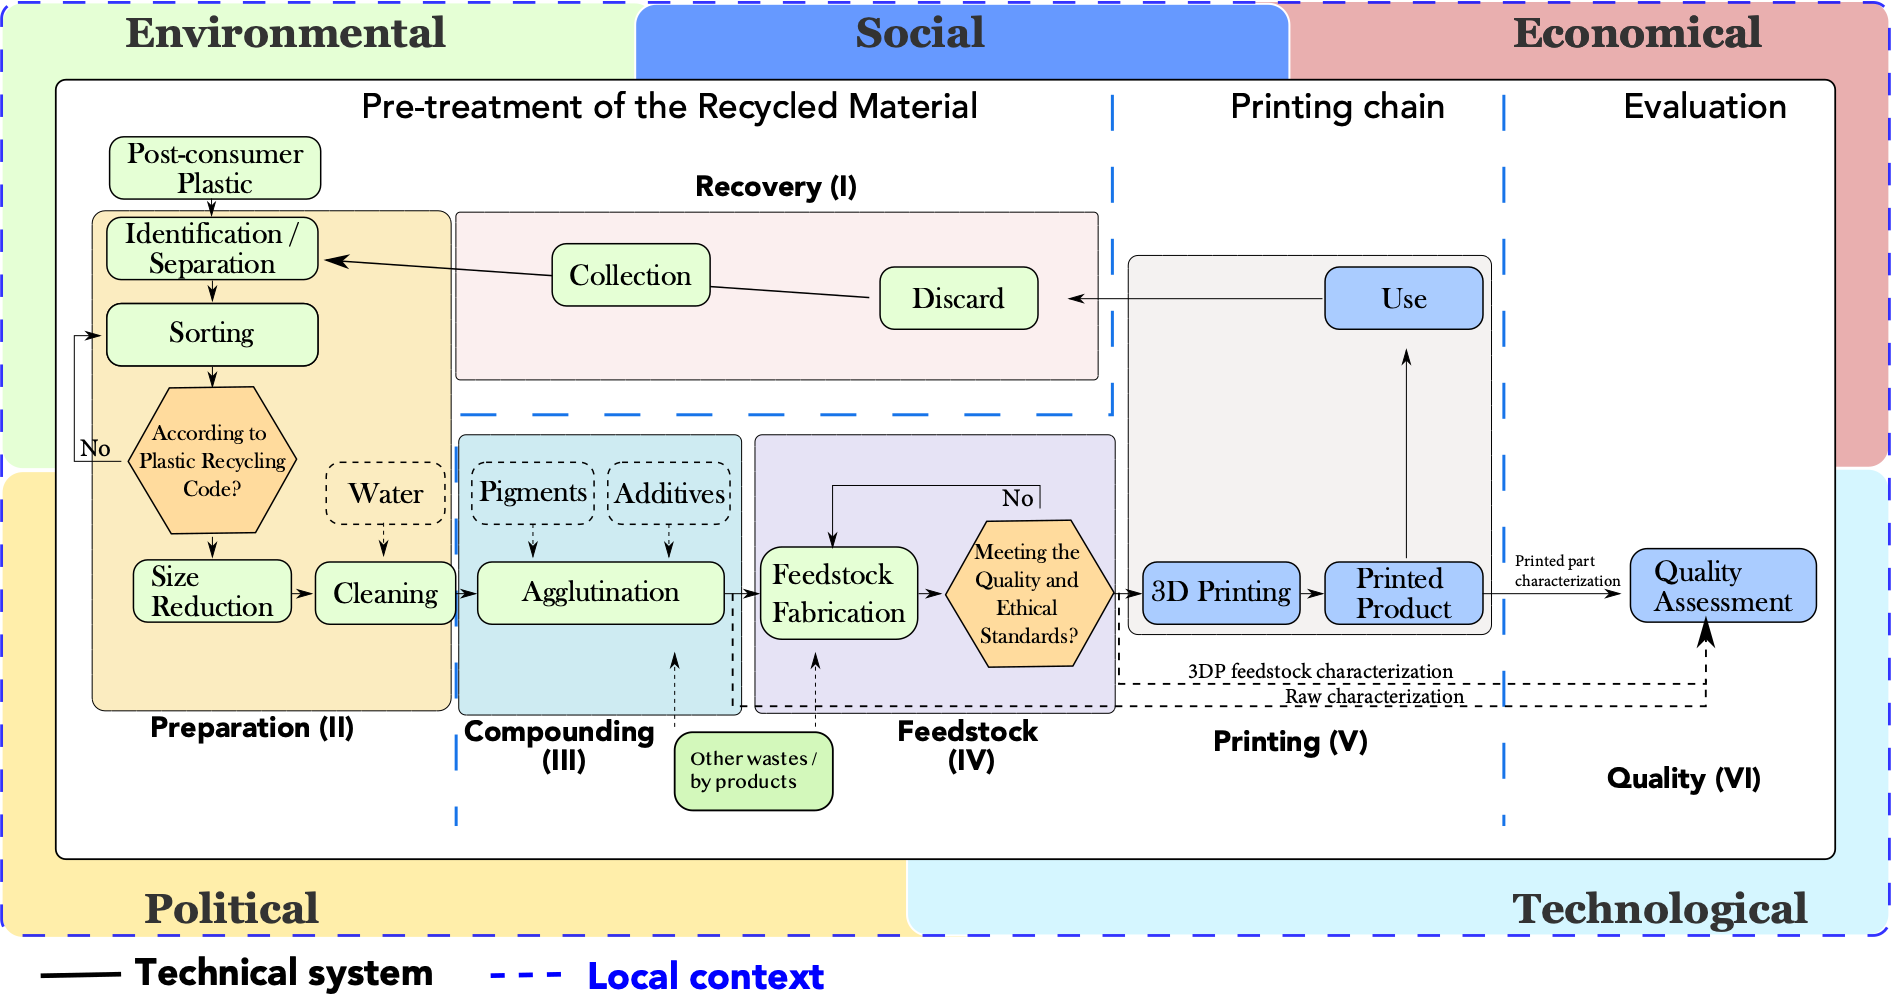
\includegraphics[width=0.9\textwidth,height=\textheight]{Figures/SDRAM-00.png}

}

\caption{\label{fig-DRAM}Distributed recycling via additive
manufacturing. Source}

\end{figure}

\hypertarget{dram}{%
\subsubsection{DRAM:}\label{dram}}

To appreciate the ground-breaking scientific nature of this idea, let me
state that the most adopted form of additive manufacturing is fused
filament fabrication, which is a material extrusion process {[}@{]}.
DRAM starts with waste plastic that is produced everywhere from
packaging to broken products. It is washed, dried and then ground or cut
into particles using a waste plastic granulator or office shredder.
Next, the particles are either converted to 3D-printing filament using a
recyclebot or printed directly. Filament made with a recyclebot costs
less than 10 cents per kg, whereas commercial filament costs \$20/kg or
more. This can produce valuable products at remarkably low costs. For
example, using a recyclebot/3D-printer combination can produce over 300
units (e.g., camera lens hoods) for the price of one such item listed on
Amazon.com. The raw material for FFF can be manufactured economically
using distributed means with a waste plastic extruder (often called a
``recyclebot'')\textsuperscript{\protect\hyperlink{ref-Baechler2013}{15}}.
Recycling of plastic waste into 3-D printing filament decreases the
embodied energy of filament by 90\% compared to traditional centralized
filament manufacturing using fossil fuels as
inputs\textsuperscript{\protect\hyperlink{ref-Kreiger2013}{16},\protect\hyperlink{ref-Zhong2017}{17}}.
Distributed recycling fits into the circular economy
paradigm\textsuperscript{\protect\hyperlink{ref-Zhong2018}{18}--\protect\hyperlink{ref-Despeisse2016}{20}},
as it eliminates most embodied energy and pollution from transportation
between processing steps. Additionaly, open-source investment should
result in an extremely high return on investment (ROI) in free and open
source
hardware\textsuperscript{\protect\hyperlink{ref-ref}{\textbf{ref?}}}.
This makes distributed recycling and additive manufacturing (DRAM)
environmentally superior to other methods of plastic recycling.

However, from a scientific perspective using a systematic literature
review, I realized that the global system maturity the technical value
chain for the implementation of a community-driven of plastic recycling
is
ambiguous\textsuperscript{\protect\hyperlink{ref-CruzSanchez2020}{21}}.
Major efforts in the scientific literature have been only concentrated
in the materials and technical validation.\\
However, the system validation remains to be difficult to implement.
More in deep, the analysis of the holistic impact that this process can
have in the context of a city remain vague, if not, not treated at all.

Moreover, I have been leading the implementation of the demostrator in
the framework of an European project. which is a sustaiability trasition
for the urban plastic in a living lab approach.

In particular, this will is important if a recycled resources industry
(RRI) is starting to conceived inside the cities. RRI is seen as driver
consists of a series of activities related to recycled resources --
e.g., recycling, refining, remanufacturing, etc. -- aspiring to mitigate
the negative externality caused by the linear
economy\textsuperscript{\protect\hyperlink{ref-wang2019b}{22}}. The
sustainable development of the RRI has thus been highlighted on many
countries' agendas to promote the circular
society\textsuperscript{\protect\hyperlink{ref-leipold2021}{23}--\protect\hyperlink{ref-jaeger-erben2021a}{25}},
as well as the goals of carbon peak and carbon neutralization. The main
difficulty remains to make affordable the use of new secondary material
applicability by the
industry\textsuperscript{\protect\hyperlink{ref-klotz2022}{26}}, but at
the end, for urban planning and polycimaking to make concrete the
ambition of circuclar economy inside the urban and regional settlements.

\hypertarget{ambition-objectives}{%
\subsection{2. Ambition \& objectives}\label{ambition-objectives}}

The material
rarefaction\textsuperscript{\protect\hyperlink{ref-hultman2021}{27}},
the ecological
integration\textsuperscript{\protect\hyperlink{ref-ref}{\textbf{ref?}}}
and the resilience of production
systems\textsuperscript{\protect\hyperlink{ref-ref}{\textbf{ref?}}}
remains a systemic problem and it calls for pushing forward the
boundaries of knowledge in the fuzzy front-end design phases of
socio-technical manufacturing configurations. There is a urgent
necessity to better understand how to develop and implement
manufacturing socio-technical demonstrators at urban levels to unleash a
sustainability transition towards appropriate and inclusive
micro-manufacturing and recycling values chains inspired on the
\emph{``Design Global / Manufacturing local'' principles}. By exploring
the case of Green Fablab At Octroi Nancy, \textbf{the purpose of SDRAM
project is create a systemic blueprint methodological approach to fully
expand the frontiers of the design socio-technical manufacturing systems
as a sustainable transitions in urban settlements.} To do so, the SDRAM
project aims to deep understanding of the three major layers and the
boundary object between them:

\begin{enumerate}
\def\labelenumi{\arabic{enumi}.}
\item
  Urban space in the lens of material rarefaction and urban
  manufacturing opportunity.
\item
  Design for open source appropriate technologies as technological
  baseline, and
\item
  Pluralism (e)valuation of socio-technical system alternative to mass
  production in frame of a urban sustainability transition.

  The ambition of this project is to open up the possibilities of a new
  field of socio-technical design of distributed and circular urban
  production systems based to the scientific community.
\end{enumerate}

\hypertarget{manufacturing-and-an-urban-priority-for-relience-and-agility.-to-develop.}{%
\paragraph{\texorpdfstring{\emph{Manufacturing and an urban priority for
relience and agility}. To
develop\ldots.}{Manufacturing and an urban priority for relience and agility. To develop\ldots.}}\label{manufacturing-and-an-urban-priority-for-relience-and-agility.-to-develop.}}

\hypertarget{the-open-source-appropriatte-technology-as-alternative-has-just-started.}{%
\paragraph{\texorpdfstring{\emph{The open-source appropriatte technology
as alternative has just
started}.}{The open-source appropriatte technology as alternative has just started.}}\label{the-open-source-appropriatte-technology-as-alternative-has-just-started.}}

In this project, the technological choices and applications that are
small-scale, economically affordable, decentralised, energy-efficient,
environmentally sound and easily utilized by local communities to meet
their needs is fundamental{[}@{]}. Therefore, the trend in appropriate
technologies is towards relatively simple and non-complex technologies,
to complete the technological mix to be capable of plastic recycling
from the identification of material, cleaning, sorting. The development
of open hardware scietnific are considered as an excellent choice to
reduce the cost {[}@{]}. The creation of a technical blueprint is there
is no a database that include is regarded as the front of A complete
technological mix aims to empower citizen in the. to To identify the
pertinent The establishment of development of a technological open
source maturity level focalised on the distributed recycling of the
design of an open source appropriate technical ecosystem (OSAT).

\hypertarget{systemic-design-thinking-to-identify-major-feedbacks-in-the-strategic-the-tactical-and-the-operational-decisional-levels.}{%
\paragraph{\texorpdfstring{\emph{Systemic design thinking to identify
major feedbacks in the strategic, the tactical and the operational
decisional
levels.}}{Systemic design thinking to identify major feedbacks in the strategic, the tactical and the operational decisional levels.}}\label{systemic-design-thinking-to-identify-major-feedbacks-in-the-strategic-the-tactical-and-the-operational-decisional-levels.}}

Reconciling urban development and industrial development is not an easy
task. Thus, the type of information that decision-makers take into
account is relevant at the moment to put in place industrial systems.

\hypertarget{pluralism-valuation-for-emerging-industrial-micro-values-chains-that-integrate-ecosystem-characteristics.}{%
\paragraph{\texorpdfstring{\emph{Pluralism valuation for emerging
industrial micro-values chains that integrate ecosystem
characteristics.}}{Pluralism valuation for emerging industrial micro-values chains that integrate ecosystem characteristics.}}\label{pluralism-valuation-for-emerging-industrial-micro-values-chains-that-integrate-ecosystem-characteristics.}}

It is urgent to expand the boundaries for engineering design from the
lowest molecular level to the process level, and from individual process
to the higher levels of value chains, ecosystems and the
planet\textsuperscript{\protect\hyperlink{ref-Martinez-Hernandez2017}{28}}.
We need to integrate ecological carrying capacity since the fuzzy front
end phase of an industrial systems. However, the integration of
ecological aspects in the decision-making seems not evident given the
complexity to define the boundaries and interactions of industrial and
ecological systems.

\hypertarget{a-challenging-task-for-a-systemic-blueprint}{%
\subsubsection{A challenging task for a systemic
blueprint}\label{a-challenging-task-for-a-systemic-blueprint}}

The major gap that currently prevents from exploring the potential of
alternative distributed manufacturing relies on a knowledge gap in terms
of the maturity in the connection between the unit-facility-urban levels
including the respective boundaries objects that needs to be considered
between the layers. From a design for
sustainability\textsuperscript{\protect\hyperlink{ref-Ceschin2016}{29},\protect\hyperlink{ref-SousaRocha2019}{30}}
perspective, this implies the aid-decision tools to help makers,
practitioners and decision-makers in the implementation phase
considering the technosphere (molecule, material, process unit) but also
the also to the ecosystem impact. Therefore as a systemic blueprint, I
aim to make linkage of the micro-meso-macro levels of the technical,
system and valuation layers embed in a urban spatio-temporal context
(See Figure network)

\hypertarget{the-methodology}{%
\subsection{3. The Methodology}\label{the-methodology}}

SDRAM implement a methodology made of four working packages (WP), as
illustrated in Fig. XXX..

The aim of WP1 is to set the literature baseline for an integrative and
critical analysis of the urban production systems integrating three
essential issues: sustainability, resiliency, and agility into a
circular economy praxis. This working package gives the insights for the
WP2, and WP3, which are key of the project. The WP2 seeks to consolidate
systematize a design for OSAT, establishing a theoretical maturity level
index that could foster the consolidatation of the OSAT in SME's. The
WP3 aims to propose a urban closed-loop system network integrating
integrates Finally, WP4 is dedicated to the experimentaiton of and
anlaysis of the several demostrators of the urban circular manufacturing
taking into case study the implementation of the Green Fablab Project at
Nancy-Fr. Workpackages are synthetically detailed hereinafter.

\hypertarget{wp-1}{%
\subsubsection{WP 1:}\label{wp-1}}

The achievement to SDRAM target relies the urban spatial characteristics
as an entry point of the design of the socio-technical system possible
identify two major output. (1.1) a predictive cartography based tool
with possible secondary materials niches at the urban level. (2.2)

\hypertarget{wp-2-maturity-level-and-technodiverstity-level-of-the-open-source-appropritte-technology}{%
\subsubsection{WP 2: Maturity level and technodiverstity level of the
open source appropritte
technology}\label{wp-2-maturity-level-and-technodiverstity-level-of-the-open-source-appropritte-technology}}

The main purpose of this task is to build a Tasks: (2.1) definition of a
Scientific literature and critical analysis on advantages and barriers
of the implications of the open-source appropritte technologies for
recycling.

\hypertarget{wp-3-systemic-analysisi-in-function-of-the-local-territory}{%
\subsubsection{WP 3: Systemic analysisi in function of the local
territory}\label{wp-3-systemic-analysisi-in-function-of-the-local-territory}}

\begin{itemize}
\tightlist
\item
  Development of methdology to identify potential urban disposal sites
  connecting
\item
  ANalyse the political, method
\end{itemize}

it is stated to analys socio-technical sytems beyond the economics
{[}@{]}, to include new form of pluralims valuation to include the
ecological interactions{[}@{]}.

\hypertarget{wp-4-pluralism-evaluation-of-the-new-alternative-manufacturing-systems}{%
\subsubsection{WP 4: Pluralism (e)valuation of the new alternative
manufacturing
systems}\label{wp-4-pluralism-evaluation-of-the-new-alternative-manufacturing-systems}}

WP4 is devoted to the implementation and experiementaiton of the
dsitributed net

To pass from ecodesign to a for design for sustainability, ten different
models at operational, tactical, and strategical levels have been
identified\textsuperscript{\protect\hyperlink{ref-SousaRocha2019}{30}}.
One strategical point in sustainability relies on the economic valuation
of ecosystem goods and services framework. This approach gives an
important framework highlighting their importance for society and human
welfare. However, there is a need to explicitly account for their
contribution when designing and developing products and
services\textsuperscript{\protect\hyperlink{ref-Diwekar2021}{31}}.

The WP4 aims to consolidate start a longitudinal study of different
initiatives of to give a to possible establish a major understanding of
the implementation

(4.1) Prospective recomendation through the participation of

\hypertarget{conceptueal-risk-and-fesability-assessment}{%
\subsection{3. Conceptueal risk and fesability
assessment}\label{conceptueal-risk-and-fesability-assessment}}

SDRAM is a high operation and conceptual-risk project mainly because as
a soio evaluation of the pactful

\hypertarget{an-impact-project}{%
\subsection{4. An Impact project}\label{an-impact-project}}

\hypertarget{resources-and-budget}{%
\subsection{5. Resources and budget}\label{resources-and-budget}}

\hypertarget{the-research-team}{%
\subsubsection{The research team}\label{the-research-team}}

The budget requied for the development of SDRAM is XXX €. The most
significant cost is the personnel cost (XXXX € - XX \%). Minor cost
cover the purchase of open hardware equipement (XXXX € - XX \%), travels
for dissemination of results (XXXX € - XX \%), Open acces fees for at
least 8 publications (XXXX € - XX \%).

\newpage

\hypertarget{references}{%
\subsection*{References}\label{references}}
\addcontentsline{toc}{subsection}{References}

\hypertarget{refs}{}
\begin{CSLReferences}{0}{0}
\leavevmode\vadjust pre{\hypertarget{ref-de-la-torre2021}{}}%
\CSLLeftMargin{1. }%
\CSLRightInline{De-la-Torre GE, Dioses-Salinas DC, Pizarro-Ortega CI, et
al. \href{https://doi.org/10.1016/j.scitotenv.2020.142216}{New plastic
formations in the {Anthropocene}}. \emph{Science of The Total
Environment} 2021; 754: 142216.}

\leavevmode\vadjust pre{\hypertarget{ref-ONeill2018}{}}%
\CSLLeftMargin{2. }%
\CSLRightInline{O'Neill DW, Fanning AL, Lamb WF, et al.
\href{https://doi.org/10.1038/s41893-018-0021-4}{A good life for all
within planetary boundaries}. \emph{Nature Sustainability} 2018; 1:
88--95.}

\leavevmode\vadjust pre{\hypertarget{ref-kanger2022}{}}%
\CSLLeftMargin{3. }%
\CSLRightInline{Kanger L, Bone F, Rotolo D, et al.
\href{https://doi.org/10.1016/J.TECHFORE.2022.121491}{Deep transitions:
{A} mixed methods study of the historical evolution of mass production}.
\emph{Technological Forecasting and Social Change} 2022; 177: 121491.}

\leavevmode\vadjust pre{\hypertarget{ref-kallis2018}{}}%
\CSLLeftMargin{4. }%
\CSLRightInline{Kallis G, Kostakis V, Lange S, et al.
\href{https://doi.org/10.1146/annurev-environ-102017-025941}{Research
{On Degrowth}}. \emph{Annu Rev Environ Resour} 2018; 43: 291--316.}

\leavevmode\vadjust pre{\hypertarget{ref-savini2021}{}}%
\CSLLeftMargin{5. }%
\CSLRightInline{Savini F.
\href{https://doi.org/10.1080/09640568.2020.1857226}{The circular
economy of waste: Recovery, incineration and urban reuse}. \emph{Journal
of Environmental Planning and Management} 2021; 64: 2114--2132.}

\leavevmode\vadjust pre{\hypertarget{ref-Riffat2016}{}}%
\CSLLeftMargin{6. }%
\CSLRightInline{Riffat S, Powell R, Aydin D.
\href{https://doi.org/10.1186/s40984-016-0014-2}{Future cities and
environmental sustainability}. \emph{Future Cities and Environment}
2016; 2: 1.}

\leavevmode\vadjust pre{\hypertarget{ref-Herrmann2020}{}}%
\CSLLeftMargin{7. }%
\CSLRightInline{Herrmann C, Juraschek M, Burggräf P, et al.
\href{https://doi.org/10.1016/j.cirp.2020.05.003}{Urban production:
{State} of the art and future trends for urban factories}. \emph{CIRP
Annals} 2020; 69: 764--787.}

\leavevmode\vadjust pre{\hypertarget{ref-sabel1985}{}}%
\CSLLeftMargin{8. }%
\CSLRightInline{Sabel C, Zeitlin J.
\href{https://www.jstor.org/stable/650576}{Historical {Alternatives} to
{Mass Production}: {Politics}, {Markets} and {Technology} in
{Nineteenth-Century Industrialization}}. \emph{Past \& Present} 1985;
133--176.}

\leavevmode\vadjust pre{\hypertarget{ref-Heikkinen2020a}{}}%
\CSLLeftMargin{9. }%
\CSLRightInline{Heikkinen ITS, Savin H, Partanen J, et al.
\href{https://doi.org/10.1016/j.techfore.2020.119986}{Towards national
policy for open source hardware research: {The} case of {Finland}}.
\emph{Technol Forecast Soc Change} 2020; 155: 119986.}

\leavevmode\vadjust pre{\hypertarget{ref-Pearce2020a}{}}%
\CSLLeftMargin{10. }%
\CSLRightInline{Pearce JM. A review of open source ventilators for
{COVID-19} and future pandemics. \emph{F1000Research}; 9. Epub ahead of
print 2020. DOI:
\href{https://doi.org/10.12688/f1000research.22942.2}{10.12688/f1000research.22942.2}.}

\leavevmode\vadjust pre{\hypertarget{ref-Ijassi2022}{}}%
\CSLLeftMargin{11. }%
\CSLRightInline{Ijassi W, Evrard D, Zwolinski P.
\href{https://doi.org/10.1016/j.procir.2022.02.048}{Characterizing urban
factories by their value chain: A first step towards more sustainability
in production}. \emph{Procedia CIRP} 2022; 105: 290--295.}

\leavevmode\vadjust pre{\hypertarget{ref-CruzSanchez2014}{}}%
\CSLLeftMargin{12. }%
\CSLRightInline{Cruz Sanchez FA, Boudaoud H, Muller L, et al.
\href{https://doi.org/10.1080/17452759.2014.919553}{Towards a standard
experimental protocol for open source additive manufacturing}.
\emph{Virtual and Physical Prototyping} 2014; 9: 151--167.}

\leavevmode\vadjust pre{\hypertarget{ref-Cruz2015}{}}%
\CSLLeftMargin{13. }%
\CSLRightInline{Cruz F, Lanza S, Boudaoud H, et al. Polymer {Recycling}
and {Additive Manufacturing} in an {Open Source} context :
{Optimization} of processes and methods. In: \emph{Solid {Freeform
Fabrication}}. {Austin, Texas}, 2015, pp. 1591--1600.}

\leavevmode\vadjust pre{\hypertarget{ref-CruzSanchez2017}{}}%
\CSLLeftMargin{14. }%
\CSLRightInline{Cruz Sanchez FA, Boudaoud H, Hoppe S, et al.
\href{https://doi.org/10.1016/j.addma.2017.05.013}{Polymer recycling in
an open-source additive manufacturing context: {Mechanical} issues}.
\emph{Additive Manufacturing} 2017; 17: 87--105.}

\leavevmode\vadjust pre{\hypertarget{ref-Baechler2013}{}}%
\CSLLeftMargin{15. }%
\CSLRightInline{Baechler C, DeVuono M, Pearce JM.
\href{https://doi.org/10.1108/13552541311302978}{Distributed recycling
of waste polymer into {RepRap} feedstock}. \emph{Rapid Prototyping
Journal} 2013; 19: 118--125.}

\leavevmode\vadjust pre{\hypertarget{ref-Kreiger2013}{}}%
\CSLLeftMargin{16. }%
\CSLRightInline{Kreiger M, Pearce JM.
\href{https://doi.org/10.1557/opl.2013.319}{Environmental {Impacts} of
{Distributed Manufacturing} from 3-{D Printing} of {Polymer Components}
and {Products}}. \emph{MRS Proceedings} 2013; 1492: 85--90.}

\leavevmode\vadjust pre{\hypertarget{ref-Zhong2017}{}}%
\CSLLeftMargin{17. }%
\CSLRightInline{Zhong S, Rakhe P, Pearce J.
\href{https://doi.org/10.3390/recycling2020010}{Energy {Payback Time} of
a {Solar Photovoltaic Powered Waste Plastic Recyclebot System}}.
\emph{Recycling} 2017; 2: 10.}

\leavevmode\vadjust pre{\hypertarget{ref-Zhong2018}{}}%
\CSLLeftMargin{18. }%
\CSLRightInline{Zhong S, Pearce JM.
\href{https://doi.org/10.1016/j.resconrec.2017.09.023}{Tightening the
loop on the circular economy: {Coupled} distributed recycling and
manufacturing with recyclebot and {RepRap} 3-{D} printing}.
\emph{Resources, Conservation and Recycling} 2018; 128: 48--58.}

\leavevmode\vadjust pre{\hypertarget{ref-Garmulewicz2018}{}}%
\CSLLeftMargin{19. }%
\CSLRightInline{Garmulewicz A, Holweg M, Veldhuis H, et al.
\href{https://doi.org/10.1177/0008125617752695}{Disruptive {Technology}
as an {Enabler} of the {Circular Economy}: {What Potential Does 3D
Printing Hold}?} \emph{California Management Review} 2018; 60:
112--132.}

\leavevmode\vadjust pre{\hypertarget{ref-Despeisse2016}{}}%
\CSLLeftMargin{20. }%
\CSLRightInline{Despeisse M, Baumers M, Brown P, et al.
\href{https://doi.org/10.1016/j.techfore.2016.09.021}{Unlocking value
for a circular economy through {3D} printing: {A} research agenda}.
\emph{Technological Forecasting and Social Change} 2017; 115: 75--84.}

\leavevmode\vadjust pre{\hypertarget{ref-CruzSanchez2020}{}}%
\CSLLeftMargin{21. }%
\CSLRightInline{Cruz Sanchez FA, Boudaoud H, Camargo M, et al.
\href{https://doi.org/10.1016/j.jclepro.2020.121602}{Plastic recycling
in additive manufacturing: {A} systematic literature review and
opportunities for the circular economy}. \emph{Journal of Cleaner
Production} 2020; 264: 121602.}

\leavevmode\vadjust pre{\hypertarget{ref-wang2019b}{}}%
\CSLLeftMargin{22. }%
\CSLRightInline{Wang M, Liu P, Gu Z, et al.
\href{https://doi.org/10.3390/ijerph16234654}{A {Scientometric Review}
of {Resource Recycling Industry}}. \emph{International Journal of
Environmental Research and Public Health} 2019; 16: 4654.}

\leavevmode\vadjust pre{\hypertarget{ref-leipold2021}{}}%
\CSLLeftMargin{23. }%
\CSLRightInline{Leipold S, Weldner K, Hohl M.
\href{https://doi.org/10.1016/j.ecolecon.2021.107086}{Do we need a
{`circular society'}? {Competing} narratives of the circular economy in
the {French} food sector}. \emph{Ecological Economics} 2021; 187:
107086.}

\leavevmode\vadjust pre{\hypertarget{ref-hobson2021}{}}%
\CSLLeftMargin{24. }%
\CSLRightInline{Hobson K, Holmes H, Welch D, et al.
\href{https://doi.org/10.1016/J.JCLEPRO.2021.128969}{Consumption {Work}
in the circular economy: {A} research agenda.} \emph{Journal of Cleaner
Production} 2021; 321: 128969.}

\leavevmode\vadjust pre{\hypertarget{ref-jaeger-erben2021a}{}}%
\CSLLeftMargin{25. }%
\CSLRightInline{Jaeger-Erben M, Jensen C, Hofmann F, et al.
\href{https://doi.org/10.1016/j.resconrec.2021.105476}{There is no
sustainable circular economy without a circular society}.
\emph{Resources, Conservation and Recycling} 2021; 168: 105476.}

\leavevmode\vadjust pre{\hypertarget{ref-klotz2022}{}}%
\CSLLeftMargin{26. }%
\CSLRightInline{Klotz M, Haupt M, Hellweg S.
\href{https://doi.org/10.1016/J.WASMAN.2022.01.002}{Limited utilization
options for secondary plastics may restrict their circularity}.
\emph{Waste Management} 2022; 141: 251--270.}

\leavevmode\vadjust pre{\hypertarget{ref-hultman2021}{}}%
\CSLLeftMargin{27. }%
\CSLRightInline{Hultman J, Corvellec H, Jerneck A, et al.
\href{https://doi.org/10.1016/j.respol.2021.104297}{A resourcification
manifesto: {Understanding} the social process of resources becoming
resources}. \emph{Research Policy} 2021; 50: 104297.}

\leavevmode\vadjust pre{\hypertarget{ref-Martinez-Hernandez2017}{}}%
\CSLLeftMargin{28. }%
\CSLRightInline{Martinez-Hernandez E.
\href{https://doi.org/10.1016/j.coche.2017.05.005}{Trends in sustainable
process design---from molecular to global scales}. \emph{Current Opinion
in Chemical Engineering} 2017; 17: 35--41.}

\leavevmode\vadjust pre{\hypertarget{ref-Ceschin2016}{}}%
\CSLLeftMargin{29. }%
\CSLRightInline{Ceschin F, Gaziulusoy I.
\href{https://doi.org/10.1016/j.destud.2016.09.002}{Evolution of design
for sustainability: {From} product design to design for system
innovations and transitions}. \emph{Design Studies} 2016; 47: 118--163.}

\leavevmode\vadjust pre{\hypertarget{ref-SousaRocha2019}{}}%
\CSLLeftMargin{30. }%
\CSLRightInline{Rocha CS, Antunes P, Partidário P.
\href{https://doi.org/10.1016/j.jclepro.2019.06.108}{Design for
sustainability models: {A} multiperspective review}. \emph{Journal of
Cleaner Production} 2019; 234: 1428--1445.}

\leavevmode\vadjust pre{\hypertarget{ref-Diwekar2021}{}}%
\CSLLeftMargin{31. }%
\CSLRightInline{Diwekar U, Amekudzi-Kennedy A, Bakshi B, et al.
\href{https://doi.org/10.1016/j.resconrec.2020.105140}{A perspective on
the role of uncertainty in sustainability science and engineering}.
\emph{Resources, Conservation and Recycling} 2021; 164: 105140.}

\end{CSLReferences}



\end{document}
